\chapter{Introducción}

Uno de los puntos más débiles en la seguridad de toda organización ha sido las contraseñas. Cuando el usuario dispone de absoluto control sobre la decisión de cómo debe ser ésta, las contraseñas tienden a ser muy débiles ante ataques de diccionario. La solución a este problema reside en el uso de políticas de contraseña que exijan unos mínimos de fortaleza (uso de minúsculas y mayúsculas, números y símbolos). Estas políticas se pueden controlar informáticamente obligando al usuario a poner contraseñas de calidad.

Por otra parte la potencia de las CPUs se ha incrementando, lo que ha supuesto la necesidad de mejorar los sistemas criptográficos para hacerlos más resistentes a todo tipo de ataques. En el caso concreto de las funciones resumen, este fortalecimiento se ha materializado de dos formas distintas:

\begin{itemize}
	\item Se ha incrementado el número de bits del resumen (para disminuir la posibilidad de colisiones).
	
	\item Se procura mejorar la técnica de generación del resumen para garantizar que los resúmenes sean lo más aleatorios posibles, utilizando procesos que impidan determinar el mensaje a partir del resumen y que garanticen estar normalmente\footnote{Si los resúmenes generados no tuviesen una distribución normal esto supondría que habría grupos de resúmenes y facilitaría ataques contra éstos pues sería más fácil determinar de dónde podrían proceder.} distribuidos. 
\end{itemize}

Estas mejoras ha ido esquivando uno de los problemas más importantes que han tenido las funciones resumen: el incremento de la potencia de las CPUs permite realizar ataques de fuerza bruta en tiempos asumibles.

El incremento de la potencia de las CPUs se ha visto restringido por la capacidad de integración de transistores en un microprocesador y el diseño interno del mismo. Si tomamos la Ley de Moore, ésta dice que el número de transistores en un microprocesador tiende a duplicarse cada 18 meses. Esto nos permite planificar qué capacidad de cómputo podría tener un CPU en el futuro de cara a evitar ataques de fuerza bruta. De todos modos, el número de transistores es solo una parte de la capacidad de una CPU ya que su estructura interna afecta también de forma muy clara. Esto se debe a la forma que tiene de organizar la ejecución de una aplicación, la calidad del predictor de saltos, etc.

Al mismo tiempo a la mejora de las CPUs, se ha ido produciendo una importante mejora en los procesadores de las tarjetas gráficas (en adelante GPU). Estos procesadores de propósito específico han visto su potencia incrementada muy rápidamente gracias a sus diseños más sencillos (se utilizan específicamente para cálculo matemático) y a su gran capacidad de paralelización (una NVIDIA Tesla puede disponer de hasta 960 núcleos) como puede verse en la Figura \ref{fig:GPUvsCPU}. Desde hace algún tiempo las tarjetas gráficas permiten cargar pequeños trozos de códigos denominados \emph{shaders} (éstos códigos se utilizan como filtros para efectos 3D) y esta técnica a desembocado en permitir la carga de códigos de usuario más genéricos.

\begin{figure}
	\centering
	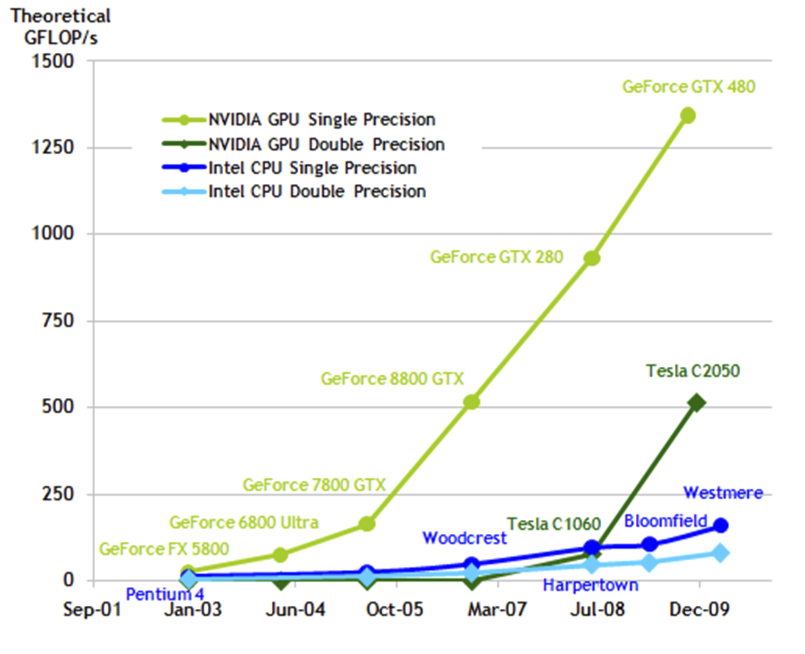
\includegraphics[width=0.7\textwidth]{images/evolucion-gpu.png}
	\caption{Comparativa de la evolución de los GFlops de las GPUs frente a las CPUs\cite{nvidia:cuda_c_programming_guide}}\label{fig:GPUvsCPU}
\end{figure}

La principal razón por la que el uso de GPU para computación se ha convertido en algo de interés es la publicación de APIs como CUDA y OpenCl que nos permiten aprovechar las capacidades de las actuales tarjetas gráficas para realizar cálculos y operaciones muy costosas en tiempo de CPU de forma más rápida. Además, permiten un alto grado de paralelismo, lo que puede resultar beneficioso para el desarrollo de ciertos tipos de programas.

En la actualidad, mientras con una CPU se podía conseguir hasta 80 millones de claves MD5 por segundo (aplicando muchas optimizaciones a nivel de lenguaje ensamblador), una GPU potente puede alcanzar hasta cerca de los 2.000 millones de resúmenes por segundo. Esto es, una GPU es hasta 250 veces más rápida que la CPU para este tipo de cálculos, propiciado, principalmente, por su mayor capacidad de paralelización.

Si consideramos el hecho de que en la actualidad casi todos los nuevos equipos que se venden en el mercado disponen de aceleradoras gráficas y que es muy fácil crear una red de ordenadores zombis se debe considerar la mejora de los mecanismos de contraseña una prioridad por parte de las organizaciones. Por este motivo es importante disponer de herramientas que permitan comprobar la fortaleza de las contraseñas y evaluar la dificultad de realizar ataques a los distintos algoritmos de resumen existentes y en experimentación.

\section{Motivación}

Como ya se ha comentado, es importante garantizar la calidad de los algoritmos que se utilizan en seguridad y las contraseñas empleadas dentro de las organizaciones. Por este motivo nace este proyecto fin de carrera que pretende ser el inicio de una herramienta versátil, sencilla y atractiva que permita ofrecer a las distintas organizaciones un mecanismo para fortalecer su seguridad. Por otra parte, el estudio del uso de tarjetas gráficas fuera del ámbito de los videojuegos y del diseño gráfico es de gran interés por la alta capacidad de cómputo que ofrecen éstas. De este modo se pretende garantizar que la amortización de los equipos informáticos es máxima ya que el aprovechamiento de los mismo será mayor. Hay que recordar que en la actualidad todos los ordenadores disponen de tarjetas gráficas con aceleración 3D y de las 3 grandes marcas del mercado (Intel, AMD y NVIDIA), dos de ellas ofrecen desde hace unos años la capacidad de ejecutar código de usuario en las mismas. En el caso de Intel, no se ofrece el uso de su GPU para cálculo, pero si permiten programar utilizando OpenCl (ver el capítulo~\ref{cap3}) para sus procesadores.

Por otra parte, la popularización de \emph{frameworks} orientados a MVC han revolucionado el mundo de la programación web. Ejemplos de ello los tenemos en Ruby on Rails, DJango o CakePHP. Lo interesante de estos \emph{frameworks} es que mejoran sustancialmente las tareas de mantenimiento de los programas web ofreciendo una serie de pautas tanto en la nomenclatura de variables y tablas de las bases de datos como en la organización que deben tener los ficheros de código fuente.

\section{Objetivos}

Para poder comprobar la fortaleza de una contraseña dada y para poder evaluar la resistencia frente a ataques de fuerza bruta de diferentes tipos de funciones resumen hace falta disponer de una herramienta adecuada. Para este fin existe una gran cantidad de herramientas, principalmente destinadas a la recuperación de contraseñas extraviadas, pero que su código es cerrado y su precio elevado. Aunque el precio puede no resultar un problema importante, consideramos que el uso de aplicaciones que no suministran su código fuente no es recomendable en el ámbito de la seguridad informática ya que es importante poder saber qué es lo que la herramienta hace y eso solo se puede determinar de forma fehaciente si ésta es de código abierto. Por otra parte, también es recomendable que la herramienta se software libre porque así, en caso de que el fabricante deje de dar soporte a la misma, tendríamos permiso para poder realizar modificaciones eliminando de este modo la dependencia con el vendedor.

El presente proyecto final de carrera nace con el objetivo de aprovechar las nuevas arquitecturas gráficas en el entorno de la evaluación de seguridad informática, especialmente en el ámbito de las funciones resumen. Igualmente se ha pretendido utilizar un modelo distribuido para mejorar la escalabilidad del sistema y así disponer de una herramienta potente que pueda ser ampliada según la necesidad del momento.

En concreto, los objetivos que se pretenden alcanzar con la realización de este proyecto son:

\begin{description}

	\item[Estudio de las distintas técnicas de evaluación de contraseñas.] Para poder garantizar la calidad de cualquier solución planteada para la evaluación de contraseñas es necesario disponer de una base suficiente sobre el tema. De este modo será más sencillo determinar si el trabajo realizado es correcto o no.
	
	\item[Aprendizaje de programación con GPU.] Esto permitirá hacer uso de un elemento de gran potencia que se encuentra hoy día en todos los ordenadores comercializados. Además, las GPU ofrecen unas características ideales para la ejecución de una gran cantidad de tareas en paralelo lo que las hace muy atractivas para realizar tareas que de otro modo podrían tardar muchísimo.
	
	\item[Utilizar nuevas técnicas de distribución de tareas.] A lo largo de la carrera se ha tratado en muchas ocasiones los sistemas distribuidos y cómo estos distribuyen su carga de trabajo entre una red de ordenadores. En este punto se pretende experimentar con algunas técnicas no tratadas o con mecanismos diferentes a los vistos.
	
	\item[Aplicar técnicas de usabilidad.] Un apartado importante de toda aplicación es la facilidad con la que esta se maneje y el grado de satisfacción del usuario de la misma. Por este motivo es importante dedicar un esfuerzo en el diseño de la interfaz y así mejorar la experiencia del usuario.
	
	\item[Ofrecer una buen grado de escalabilidad.] Gracias a esto se pretende conseguir que el sistema desarrollado puede crecer con el tiempo de forma sencilla introduciendo nuevos ordenadores. De este modo se reducirían los costes al no tener que comprar grandes sistemas exclusivamente para este propósito.
	
	\item[Garantizar que la herramienta desarrollada sea mantenible.] Para ello es necesario hacer un buen uso de los comentarios y se debe garantizar que estén bien documentados los aspectos más importantes de diseño de la herramienta. De este modo se conseguirá que en un futuro cualquier persona puede realizar modificaciones sobre la misma en caso de fallos.
	
	\item[Implementar un sistema de extensiones.] Con esto se pretende que la herramienta pueda ver ampliada su funcionalidad sin necesidad de que deba ser compilada nuevamente. Para ser más exactos, lo que se pretende es que durante el inicio de la ejecución de la herramienta esta busque en el sistema extensiones que le añadan funcionalidades.
	
	\item[Crear un mecanismo sencillo de administración.] De este modo se pretende mejorar el tiempo requerido para la realización de las tareas relacionadas con la aplicación.
	
	\item[Desarrollo de una interfaz web.] En la actualidad casi todos los equipos informáticos se encuentran conectados, sino a Internet, sí a una red de ordenadores. Por norma general los cortafuegos empresariales filtran el tráfico que circula por la red, pero permiten el uso de Web lo que convierte a la Web casi en el medio exclusivo para usarlo como protocolo para la administración remota.
	
	\item[Uso de los \emph{frameworks} MVC.] Con esto se pretende garantizar la mantenibilidad de la solución web anteriormente comentada. Además, el uso de \emph{frameworks} ya existentes facilitan el mantenimiento de la aplicación ya que solo habrá que dedicar esfuerzo al desarrollo de la herramienta y en caso de mejoras en el \emph{framework} éstas se pueden ver inmediatamente reflejadas en la aplicación sin apenas tener que realizar cambios (en muchos casos no es necesario realizar cambio alguno).
\end{description}

\section{Estructura del documento}

Para facilitar la búsqueda a través del este documento, se provee de la siguiente guía de la organización interna del mismo. Éste se divide en los siguiente capítulos:

\begin{description}
	\item[Funciones resumen:] introducción a las funciones resumen y a los tipos de ataques que existen sobre ellas. Es importante comprender qué son para entender mejor cuales son los objetivos del proyecto.
	
	\item[Desarrollo con tarjetas gráficas:] se introduce la historia del desarrollo con tarjetas gráficas y a cómo se programa utilizando CUDA, el API de NVIDIA. Con esto se pretende ofrecer una visión global sobre el uso de tarjetas gráficas y el porqué de su uso.
	
	\item[Mejora de una aplicación distribuida:] se muestra un estudio sobre una aplicación ya existente y los cambios que se le han realizado y las motivaciones para ello.
	
	\item[Resultados:] se enumeran las pruebas y los resultados obtenidos por las mismas.
	
	\item[Conclusiones:] conclusiones obtenidas de la realización del proyecto en las que se intenta valorar el grado de consecución del mismo.
	
	\item[Trabajos futuros:] descripción de posibles trabajos futuros que sería interesante realizar a partir del trabajo realizado en este proyecto final de carrera.
\end{description}